\documentclass[journal,onecolumn]{IEEEtran}

\usepackage{cite}
\usepackage[pdftex]{graphicx}
\usepackage[cmex10]{amsmath}
\interdisplaylinepenalty=2500
\usepackage{array}
\usepackage{url}
\usepackage{fancyvrb}
\usepackage{color}
\usepackage[ascii]{inputenc}
\usepackage{listings}
\lstset{language=Python,
        numbers=left,
        keywordstyle=\color[rgb]{0,0,1},
        commentstyle=\color[rgb]{0.133,0.545,0.133},
        stringstyle=\color[rgb]{0.627,0.126,0.941},
        columns=fixed,}

\markboth{EE643}{Jonathan Klein}


\begin{document}
\title{Parallelized Viterbi Algorithm in Python using PyCUDA and PP}
\author{\IEEEauthorblockN{Jonathan Klein}\\
    \IEEEauthorblockA{Department of Electrical and\\Computer Engineering\\
    University of Alaska, Fairbanks\\
    Fairbanks, Alaska 99775, USA\\
    Email: kleinjt@ieee.org}}


\maketitle

\begin{abstract}
%\boldmath
Pyterbi is an open source Viterbi decoder parallelized either with CUDA or SMP. It is written in Python and uses the PyCUDA and PP modules. The PyCUDA parallelized Viterbi decoder is approximately 100 times faster than the single core unparallelized reference implementation. Each probable path at each state is computed in parallel, and the backtraces of multiple trellises is computed in parallel. The PP parallelized path can process multiple Viterbi trellises simultaneously and can dispatch them across multiple cores or computers.  

\hfill \today 
\end{abstract}

\section{Introduction}
Pyterbi is an open source parallelized Viterbi decoder. It is capable of finding the most likely sequence of states through an arbitrary number of probabilistic finite state machine given noisy output observations. The PyCUDA parallelized path computes extracts parallelism by computing the most likely previous state for each possible state every time step in parallel. The PP parallelized path dispatches trellises to multiple CPU cores or servers over a network.


Viterbi decoders have applications to pattern recognition and communication systems, including speech recognition, convolution code decoding, and continuous phase modulation decoding [1] [2]. A parallelized Viterbi decoder could be useful for wireless base stations communicating with many devices using convolutional coding or continuous phase modulation or a call center performing voice recognition on several incoming calls. More realistically, pyterbi provides an open source example of PyCUDA, PP, and generating graphs using matplotlib.   


The Viterbi algorithm maintains the most likely sequence of states leading to state. This is repeated for each observation. See Figure 2 for the reference Python implementation of the forward pass of the Viterbi algorithm.
\begin{figure}[h!]
\begin{lstlisting}
# set initial probabilities
path_p[0,:] = init_p + emit_p[obs[0]]

for n in range(1, nobs):
    for m in states:
        # calculate probabilities of previous states transitioning to state m    
        p = emit_p[obs[n]][m] + trans_p[:,m] + path_p[n-1]
        # select most likely previous state for state m
        back[n][m] = numpy.argmax(p)
        # set that as probability of state m at time n 
        path_p[n][m] = numpy.amax(p)
\end{lstlisting}
    \label{fig:forcode}
    \caption{Python code for Viterbi forward path.}
\end{figure} 

Once the most likely prior state for each state and observation in the trellis has been tabulated, the most likely path through a trellis can be computed. Starting with the most likely final state, the most likely sequence of states can be traced back through the trellis. See Figure 2 for Python code implementing the backwards pass of the Viterbi algorithm. 
\begin{figure}[h!]
\begin{lstlisting}
route = numpy.zeros(nobs,dtype=numpy.int16)
# find the most likely final state
route[-1] = numpy.argmax(path_p[-1,:])

for n in range(2,nobs+1):
    # backtrace through trellis selecting the most likely previous trace
    route[-n] = back[nobs-n+1,route[nobs-n+1]]
\end{lstlisting}
    \label{fig:backcode}
    \caption{Python code for Viterbi backtrace.}
\end{figure}

\section{Hardware Platform}
Pyterbi was tested on a Lenovo T420-41786VU laptop. This platform has a few limitations which add uncertainty to the benchmarks. 

\subsection{Host Processor}
The Intel i5-2520M processor supports Intel Turbo Boost, which dynamically scales core frequencies to maintain temperature limits [4]. This means that an application running on one core could see higher clock frequencies than an application which keeps two cores active. Additionally, the T420 laptop can't sustain full processor usage on both cores for an extended period of time. The laptop provided warning messages to a terminal stating that processor speed was being scaled back to avoid overheating while running an extended PP benchmark. These factors will increase the relative performance of shorter single core tasks.  

    \begin{figure}[!h]
            \begin{tabular}{ | l | l |}
                \hline
                Processor & Intel i5-2520M, 2.50GHz \\ \hline
                Cache & 3MB Cache \\ \hline
                Cores & 2 Hyper-Threaded cores \\ \hline
                Memory & 4096MB RAM \\ \hline
                OS & Linux 2.6.38-10 \\ \hline
            \end{tabular}
    \end{figure}
    
\subsection{Graphics Card}
    PyCUDA was written and tested on a NVIDIA NVS4200M graphics card. This is a low-end laptop graphics card with only a 64-bit memory bus and 48 cores. Performance of pyterbi would probably increase on a higher performance desktop graphics card. 
     \begin{figure}[!h]
            \begin{tabular}{ | l | l |}
                \hline
                Graphics Card& Nvidia NVS 4200M \\ \hline
                Memory & 1024 MB DDR3\\ \hline
                CUDA Cores & 48 \\ \hline
                Memory Bus Width & 64 bits\\ \hline
                Driver & 270.41.19 \\ \hline
                CUDA Version & 4.0 \\ \hline
                Core Speed & 800 MHz \\ \hline
                Device to Host Bandwidth & 2600MB/s \\ \hline
                Host to Device Bandwidth & 3000MB/s \\ \hline
                Compute Capability & 2.1 \\ \hline
            \end{tabular}
    \end{figure}

\section{Parallelization}
        The PyCUDA path of pyterbi was parallelized by computing the most likely previous state for each state in parallel for an observation. This is equivalent to parallelizing the for loop on line 5 of Figure 1. These can be computed in parallel, because each state only depends on information from previous observations. See Figure~\ref{fig:cpm} for an illustration of this. In this this figure, each thread is represented by a color, and lines represent accessing the probability of prior states. The treads are synchronized at every observation after computing the most likely previous state. Each trellis is mapped to a block of threads, which can share a grid with other trellises. 

        \begin{figure}
            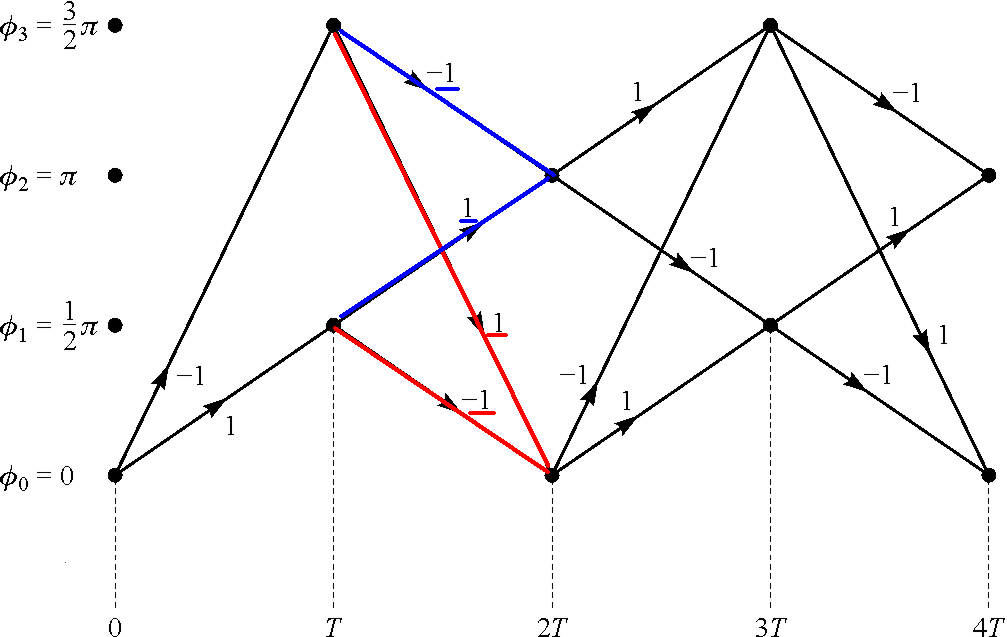
\includegraphics[width=.8\textwidth]{figures/cpmfulltrelliscolored.png}
            \caption{Viterbi algorithm at time T=2Ts. Figure adapted from Proakis [2].}
            \label{fig:cpm}
        \end{figure}

The PP path is parallelized by dispatching processes to compute each trellis. This is coarser parallelism than the PyCUDA path. Finer grained parallelism was not easily possible using the standard Python interpreter because of the global interpreter lock, which prevents concurrent execution of multiple threads. Processes are more expensive to create than threads and cannot share memory as easily, so instead of creating threads for each state in a trellis, the PP path of pyterbi creates a process for each trellis.    

\section{Software Design and Data Location}
The first version of the PyCUDA path of pyterbi was 15 times faster than the reference path. Many optimizations and tweaks later, this was improved to a 100 times speedup. 
        
The first optimization of pyterbi was moving the emission probability, observation, and transmission probability matrices from global to constant memory. This slowed down execution time by 50\%. This is possibly due to stuffing too much information into the constant cache and ignoring the L1/L2 cache present for global memory on compute capability 2.1 cards. Moving only the observation sequence to constant memory increased execution by 5\%. Eventually, the observation sequence and all other constant information was cached in shared memory instead of constant memory to support an arbitrary number of trellises.

The next optimization to Pyterbi was caching the emission probability, observation, and transmission matrices in shared memory. These matrices are filled from global memory at the start of the kernel in parallel, with a coalesced memory access pattern. Caching the constant matrices in shared memory at the start of each kernel reduced execution time by another 5\%. In addition to caching constant information in shared memory, the slices of the probability matrix representing the current and previous state probabilities are stored in shared memory.

The largest speed up for the PyCUDA path of pyterbi came from reducing communication between the host and graphics card. The initial version of pyterbi called a kernel for each observation, implicitly synchronizing. Moving the observation loop to the kernel and explicitly synchronizing threads in a kernel reduced the number of kernel calls from the number of observations to once per trellis, which led to over a 100\% speedup.

The final optimization to pyterbi was moving the backtrace computation from the host to the device. This meant the backtrace of multiple trellises could be computed in parallel, and only the route information needs to be copied back to the host for each trellis, instead of copying back the final path probabilities and the entire backtrace matrix, which is much larger. Optimizing the backtrace led to a 40\% speedup.

\section{Results}
The SMP PP path of pyterbi approaches a two times speedup on a dual core hardware platform as the complexity of a trellis increases. See Figure \ref{fig_rhost} for a plot of the speedup of the PP path across observation sequence lengths and number of states. The speedup may be approaching two for more complicated inputs because the constant time associated with creating and dispatching jobs becomes dwarfed by time spent processing the trellises. The speedup will probably approach four on a four core processor given a sufficiently large number of complex trellises.

\begin{figure*}[!t]
    \centering
    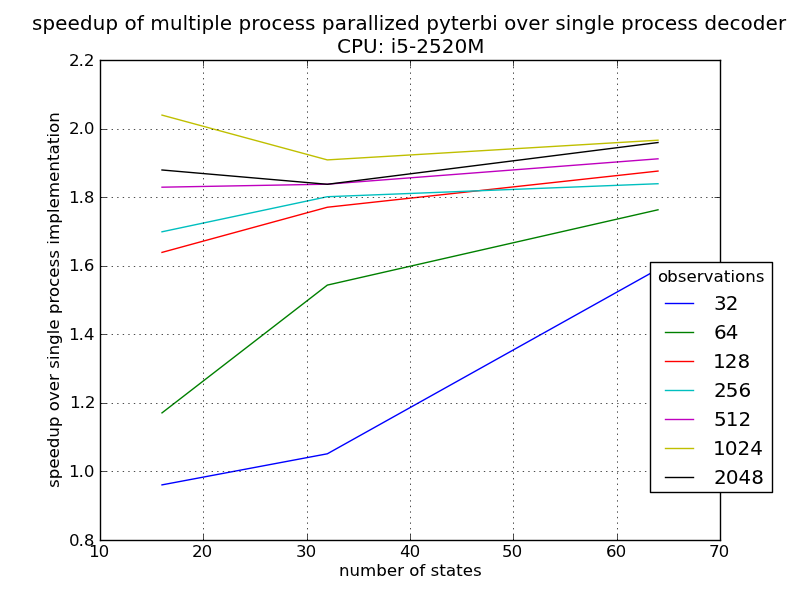
\includegraphics[width=.5 \linewidth]{figures/speedupgraphhost.png}
    \caption{Speedup of multiple process parallelized pyterbi over a single process decoder.}
    \label{fig_rhost}
\end{figure*}

In addition parallelizing for multiple core processors, PP also allows parallelization on clusters of computers. As a proof of concept, I tested pyterbi in a cluster consisting of a T420 laptop connected to a low-end VPS sharing a single AMD Opteron core with an unknown number of other virtual machines through a tethered internet connection from a cell phone. Clustering a single core of the T420 with the server led to a 10\% speedup. The speedup would probably be improved by using a cluster of faster computers connected with a more suitable network connection.

The PyCUDA path of pyterbi provides over 100 times speedup compared the reference implementation for sufficiently complex trellises. See Figure \ref{fig_rcuda} for a graph of PyCUDA speedup as the observation length and number of states increases. The speedup generally increases as the observation length increases, and as the number of states in the trellis increases. This is probably because the increased complexity with an increase in states is $O(N)$ for the PyCUDA path, and $O(N^2)$ for the reference path. The speedup also increases as the observation length increases. This is probably because the relatively constant setup time of creating and initializing the kernel is overtaken by the time spend traversing the trellis.

\begin{figure*}[!t]
    \centering
    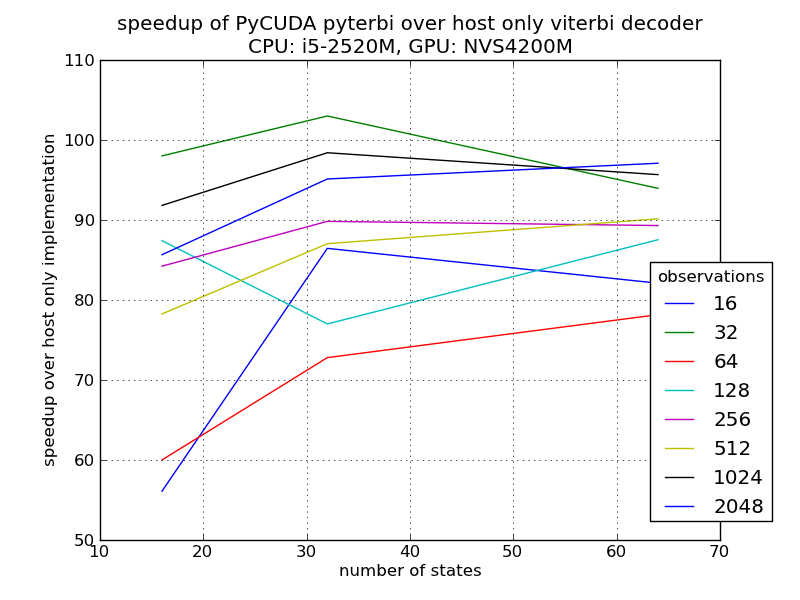
\includegraphics[width=.5 \linewidth]{figures/speedupgraphcuda.png}
    \caption{Speedup from CUDA parallelized viterbi decoder.}
    \label{fig_rcuda}
\end{figure*}


\section{Conclusion}
Pyterbi achieves a noticeable speedup over a non-parallelized reference implementation. It provided an opportunity to learn about CUDA and the PyCUDA and PP libraries. 
Several improvements to pyterbi are possible:
\begin{itemize}
    \item Rewriting the host code in a faster language (C)
    \item Rewriting host code for finer-grained parallelism with threads
    \item Testing kernel concurrency on more powerful graphics cards
    \item Testing realistic cases of cluster computing
    \item Getting PyCUDA working with PP for CUDA accelerated cluster computing 
\end{itemize}

PyCUDA made accessing the CUDA API more pleasant than using CUDA from C. Abstracting away the cleanup of objects, error checking, and some of the syntax for memory transfers was helpful. While it doesn't save the programmer from understanding what is happening (and the kernel must still be written in C), it makes programming and debugging faster and easier. Learning CUDA through PyCUDA is a little more gentle. Likewise, the PP module was impressive. Easy to use parallelism libraries for higher level languages make parallel programming very accessible, and reduce the cost of parallelizing suitable applications.

All the source code from this project, including this paper, are available under an MIT license at \url{http://github.com/loxodes/pyterbi}

\section*{References}
        [1] Lou, H.-L.; , ``Implementing the Viterbi algorithm,'' Signal Processing Magazine, IEEE , vol.12, no.5, pp.42-52, Sep 1995 \\

        [2] John Proakis. Digital Communications. McGraw-Hill Science/Engineering/Math, 5 edition, 2007. \\

        [3] C. Liu, ``CuHMM: a CUDA Implementation of Hidden Markov Model Training and Classification,'' 2009 \\

        [4] Intel, ``Intel Turbo Boost Technology 2.0,'' 2011, URL: \url{http://www.intel.com/content/www/us/en/architecture-and-technology/turbo-boost/turbo-boost-technology.html}\\

        [5] Vanovschi V., ``Parallel Python Software,'', 2011, \url{http://www.parallelpython.com}\\

        [6] Andreas Kloeckner, ``PyCUDA,'', 2011, \url{http://mathema.tician.de/software/pycuda}\\

\end{document}
